\documentclass{report}
 
\usepackage[utf8]{inputenc} 
\usepackage[T1]{fontenc}      
\usepackage[top=3.5cm, bottom=3cm, left=4.0cm, right=4.0cm]{geometry}
\usepackage{graphicx}
\graphicspath{{figures/}{../figures}}

\begin{document}

\chapter{Fonctions de transfert, AO en régime linéaire}

\newpage

\section*{Questions de cours}
\begin{itemize}

	\item[•] Énoncez les formes canoniques des filtres passe-bas, passe-haut et passe bande d'ordre 2. Pour ce dernier, tracez le diagramme de Bode en fonction des différentes paramètres.
	
	\item[•] Quelles sont les caractéristiques d'un AO idéal ?

	\item[•] Donnez le schéma de montage d'un \textbf{amplificateur non inverseur} en précisant la fonction de transfert.
	
	\item[•] Qu'est-ce qu'un circuit stable ? Quel est le critère de stabilité pour un quadripôle d'ordre 2 en régime libre (c'est-à-dire quand on branche la sortie sur l'entrée) ?

\end{itemize}

\section*{Exercices supplémentaires (difficile)}

\begin{itemize}

	\item[•] Comment réaliser une source de courant parfaite ?
	
	\item[•] Dans un montage amplificateur non-inverseur, comment minimiser la puissance dissipée par l'amplificateur opérationnel ?

\end{itemize}

\newpage

\section*{Exercice 1}
 
On souhaite alimenter un dispositif électrique (en rouge) modélisé par une résistance de charge $R_c$ avec une tension nominale $V_{nom}$. On dispose pour cela d'une source de tension (en bleue) mais dont la tension de sortie maximale $V_{max}$ est $V_{max} = V_{nom}/2$, insuffisante pour l'usage voulu.

On introduit un montage intermédiaire pour compenser l'insuffisance de la source. 

\begin{itemize}
	\item[•] Calculer $U_s$ en fonction de $U_e$ et déterminer le rôle de ce montage. Comment doit-on choisir $R_1$ et $R_2$ pour que $U_s = V_{nom}=2V_{max}$ ?
	\item[•]  On suppose dans un premier temps que $R_c=\infty$, cad que la résistance de charge n'est pas connectée au circuit. Quelle est la puissance électrique émise par l'AO ?
	\item[•] On suppose maintenant que le circuit est connecté à la charge, cad que $R_c$ est finie. Quelle est désormais la puissance dégagée par l'AO ?
	\item[•] Comment choisir $R_1$ et $R_2$ de sorte à minimiser la puissance sortie par l'AO ?
\end{itemize}

\begin{figure}[!h]
\centering
\includegraphics[width=0.5\linewidth]{puissance_AO.pdf}
\end{figure}

\newpage

\section*{Exercice 2}
Déterminer la fonction de transfert de ce filtre, que l'on mettra sous lal forme suivante : 
\begin{equation}
\underline{H}(j\omega) = H_{0}\frac{\prod_{k=1}^{n} (1+j\omega/\omega_{k})}{\prod_{l=1}^{m} (1+j\omega/\omega_{l})}
\end{equation} 

Tracer le diagramme de Bode correspondant en fonction des différentes pulsations en jeu. Expliciter trois cas possibles.

\begin{figure}[!h]
\centering
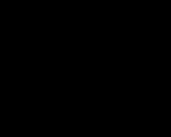
\includegraphics[width=0.5\linewidth]{circuit_6.pdf}
\end{figure}

 \newpage

\section*{Exercice 3}

Après avoir précisé le comportement du circuit en basse et haute fréquence, déterminez la fonction de transfert de ce filtre sous la forme canonique. Quel est le rôle de ce filtre ? Tracez le diagramme de Bode correspondant et déterminez sa bande passante. 

\textit{Données : $R=50k\Omega$ et $C=3.2nF$}

\begin{figure}[!h]
\centering
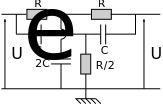
\includegraphics[width=0.5\linewidth]{circuit_2.pdf}
\end{figure}

\section*{Question supplémentaire}
On suppose désormais que $R=50k\Omega$ et $C=3.2nF$. On envoie un signal de fondamental $f_{0}=1kHz$ dont le développement en série de Fourier est donné par :
\begin{equation}
u_{e}(t)=\frac{4E}{\pi}\sum_{p=0}^{\infty}\frac{\sin \left[    \left( 2p+1\right)2\pi f_{0}t \right]}{2p+1}  
\end{equation}

Quel est ce signal ? Quel est l'effet du filtre sur ce signal ? On tracera schématiquement le signal d'entrée et de sortie.

\newpage

\section*{Exercice 4}
\begin{itemize}
\item[•] Explicitez la fonction de transfert de ce filtre, puis calculez son gain et sa phase. On notera $\omega_0$ sa pulsation caractéristique. Quel est son rôle ?
\begin{figure}[!h]
\centering
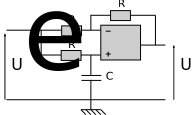
\includegraphics[width=0.5\linewidth]{circuit_.pdf}
\end{figure}

\item[•]
Pour quelles conditions sur le circuit et le signal d'entrée trouve t-on que le circuit retarde un signal périodique sans le déformer, c'est-à-dire que $U_{s}(t)=U_{e}(t-\tau)$ ? Exprimez alors ce retard $\tau$ en fonction de $R$ et $C$.
\textit{Conseil : utiliser la décomposition spectrale d'un signal}
\item[•] On envoie en entrée le signal suivant :
\begin{equation}
U_{e}(t) = U_{0}\cos^{3}(\omega t)
\end{equation}
En décomposant $U_e(t)$ en une somme de deux signaux, écrire l'expression de $U_s(t)$, le signal en sortie du filtre.

Décrire l'effet du filtre sur ce signal pour $\omega = \frac{\omega_{0}}{3}$ et $\omega=10^{-2}\omega_0$.

\item[•]
On suppose le condensateur déchargé à $t=0$. On envoie un échelon de tension $E$ en entrée. Quelle est la sortie ? Commenter.
\end{itemize}

\newpage

\section*{Exercice 5}

On considère le montage ci-dessous :
\begin{figure}[!h]
\centering
\includegraphics[width=0.5\linewidth]{derivateur.pdf}
\end{figure}
\begin{itemize}
	\item[•] On suppose dans un premier temps que l'AO est idéal. Qu'est-ce que cela signifie ? Calculez la fonction de transfert de ce montage. Quel est son rôle ?
	\item[•] On suppose désormais que l'AO est réel. On suppose alors que la sortie $u_s$ est reliée à $\varepsilon=u_+-u_-$ par la relation :
	\begin{equation}
		\tau\frac{du_s}{dt} +u_s = \mu_0\varepsilon
	\end{equation}
	avec $\mu_0=10^5$ et $\frac{\mu_0}{2\pi\tau}=$1MHz.
	
	Quel est la nouvelle fonction de transfert ? 
	
	Le montage est il stable ?
	
	\item[•] Que se passe t-il si l'on intervertit les bornes + et - de l'AO ?
	
	\item[•] A quel type de montage ce circuit s'apparente t-il ? Calculez ses caractéristiques pour $R=10$k$\Omega$ et $C=$100nF. Pour quelle fréquences agit-il comme un dérivateur ? 
\end{itemize}

\end{document}
